\chapter{Vizualizace dat}
\label{ch:vizualizace}

Očištěná data vybrané společnosti obsahující záznamy shrinků, jsem vizualizovala v~nástroji Power BI, který se používá pro business intelligence analýzu. Vizualizace se týká pouze těch shrinků, které spadají do kategorie \emph{shrinky způsobené škodami}, přehled dělení shrinků se nachází v~části \label{sec:shrinkyTypy}
. Vytvořila jsem report, který umožňuje pomocí interaktivních grafů analyzovat data. První část této kapitoly se věnuje technickému popisu reportu, zatímco druhá část shrnuje výsledky analýzy plynoucí z~reportu.

\section{Popis řešení}
\label{sec:vizualizace:popis}

Report obsahuje pět stránek. První stránka nabízí základní přehled, dashboard, týkající se všech shrinků. Druhá stránka je věnována prodejnám a údajům o lokalitách.
Další stránky se již věnují pouze shrinkům zaviněných škodami a kategoriím Velmi čerstvé a Čerstvé z~produktové hierarchie úrovně 1. Třetí stránka zobrazuje hodnoty ukazatelů hodnoty shrinku a odvozených podílů. Na čtvrté a páté stránce jsou další přehledy z~pohledu konkrétních produktů, kategorií a typů promoakce. Poslední stránka týkající se reportingu je z~pohledu vybraného konkrétního produktu.

Do Power BI souboru jsem pomocí integrovaného nástroje PowerQuery nahrála upravená data z~databáze vybrané společnosti. Hlavní faktickou tabulkou je tabulka \emph{damages}, která obsahuje všechny zaznamenané shrinky z~kategorie shrinků, které byly způsobeny škodami. Druhá faktická tabulka má název \emph{revenue} a obsahuje tržby v~pozorovaném měsíci pro všechny prodejny, tržby jsou dále rozdělené podle kategorie z~úrovně 1 a do čtvrtin měsíce. Doménové tabulky jsou číselník produktů, číselník shrinků a číselník prodejen, dále také číselníkové tabulky, které spojují faktické tabulky -- čtvrtina měsíce a seznam kategorií úrovně 1. 

Datový model tabulek, které jsou vstupem do reportu je znázorněný na obrázku \ref{obr:datmod}. Mezi jednotlivými tabulkami jsou znázorněny vazby -- jejich mohutnost a směr. Tabulka \emph{metrics}, která není navázaná na žádnou jinou tabulku obsahuje výpočetní metriky, které vychází z~dat v~modelu, metriky se dále používají ve vizualizacích.

\begin{figure}[h!]
    \centering
    \captionsetup{justification=centering}
    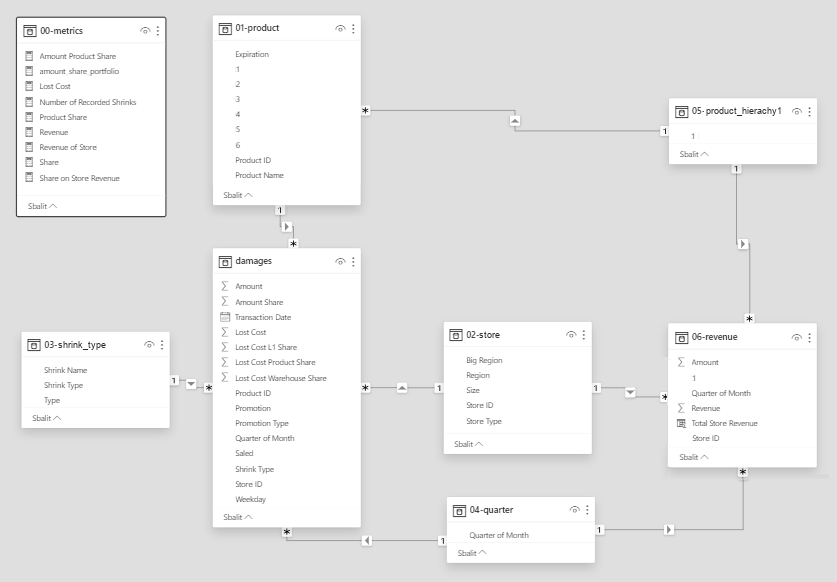
\includegraphics[width=\textwidth]{obrazky/PBI/datmodel.png}
    \caption{Datový model tabulek v~Power BI reportu.}
    \label{obr:datmod}
\end{figure}

Reporting je zpracován v~angličtině, takže i dříve popsané názvy kategorií nebo shrinků jsou přeložené. Překlad je uvedený v~příloze práce. Uvedené tržby v~reportingu odpovídají nekonkrétní peněžní jednotce -- z~důvodu ochrany dat vybrané společnosti byla skutečná čísla vynásobena jistým koeficientem. Poměry zobrazené v~reportu ale vstupním datům společnosti odpovídají.

\subsection{Metriky}

Power BI nabízí uživatelům reportu širokou interakci s~vizuály. Díky metrikám se zobrazené hodnoty přepočítávají podle aktuálních filtrů nebo podle vybraných dat. 

\begin{itemize}
    \itemsep-0.3em
    \item     \textbf{Lost Cost} -- Základní metrika s~hodnotou shrinku ze vstupních dat.
    \item     \textbf{Product Share} -- Základní metrika, obsahuje podíl shrinku na tržbách produktu (přímo ze vstupních dat). Pokud je ve vizuálu agregovaná např. na kategorii nebo prodejnu, vypočítá se její průměr.
    \item     \textbf{Share} -- Základní metrika, obsahuje podíl shrinku na tržbách produktu. Pokud je ve vizuálu agregovaná na prodejnu jedná se celkový evidovaný shrink prodejny dělený tržbou dané prodejny. Pokud je agregovaný podle typu shrinku jedná se o podíl součtu hodnot všech záznamů daného typu a tržeb všech prodejen. Bude-li agregace probíhat zároveň na typu shrinku a na kategorii z~úrovně 1, pak je podíl spočítaný vzhledem k~této kategorii typu shrinku zároveň. 
    \item     \textbf{Share on Store Revenue} -- Základní metrika, obsahuje podíl shrinku na celkových tržbách produktu. Tj. pokud je agregace např. podle prodejny a podle kategorie jedná se o podíl všech shrinků produktu z~dané kategorie vydělený celkovými tržbami vybrané prodejny. (Zatímco v~předchozí metrice by se jednalo o tržby pouze za vybranou kategorii.)
    \item     \textbf{Revenue of Stores} -- Celková tržba prodejny za celé sledované období
    \item     \textbf{Revenue} -- Základní metrika s~hodnotou tržeb prodejny rozdělená podle části měsíce podle kategorií z~úrovně 1 a  ze vstupních dat.
    \item     \textbf{Number of Recorded Shrinks} -- Počet záznamů shrinků.
\end{itemize}

\subsection{Reporting}

\subsubsection*{Přehled}

První stránka obsahuje přehled týkající se všech typů shrinků v~rámci kategorie shrinky způsobené škodami, přehled je v~tabulce \ref*{tab:sh:dam} v~kapitole \ref*{ch:shrinky}. Na obr.~\ref*{obr:PBI:overview} je snímek této stránky, pro lepší orientaci při popisu jsem na snímek přidala označující čísla. Na této stránce jsou vyfiltrované všechny kategorie, shrinky i prodejny. V~levé části jsou uvedeny souhrnné informace pro vyfiltrované záznamy (tj. implicitně nic vyfiltrováno není, jedná se o celkové hodnoty) (č. 1). 

Na grafu označeném č. 2, je znázorněno jak velký podíl shrinku na tržbách mají jednotlivé kategorie. Zároveň je barevně označeno, jakou měrou je hodnota zastoupená na malých či velkých prodejnách. Defaultní nastavení vizuálu je zobrazení kategorií úrovně 1, díky funkcionalitě nástroje Power BI je možné postoupit v~hierarchii kategorií níže viz \ref*{obr:PBI:drill}. První graf zobrazuje defaultní pohled, na druhém je vidět výsledek pokud uživatel klikne na ikonu $\downdownarrows$ \emph{přechod k~podrobnostem všech polí}. V~takovém případě se postoupí na další úroveň hierarchie napříč všemi kategoriemi. Třetí graf ukazuje stav, kterého uživatel docílí, pokud zaklikne ikonu $\downarrow$ \emph{přechod k~podrobnostem jednoho pole}\footnote{Anglicky se přechod k~podrobnostem jednoho pole v~nástroji Power BI označuje jako \emph{drill down}.}. V~takovém případě, poté co uživatel klikne na jednu z~kategorií v~grafu (její název nebo příslušný datový pruh), se zobrazí nižší úroveň hierarchie, ale pouze takové kategorie, které jsou podkategorií vybrané kategorie. 
Další graf (č. 3) ukazuje jaký je podíl shrinku na tržbách pro malé a velké prodejny. V~tomto vizuálu po zvolení přechodu k~podrobnostem se rozbalí hodnoty podílu pro jednotlivé typy shrinků. Opět jako v~předchozím případě lze postupovat buď pouze pro jeden typ prodejen nebo oba.
Pokud uživatel nezvolí \emph{přechod k~podrobnostem jednoho pole} ve vizuálu, ale klikne na datový element ve vizuálu, všechny vizuály na stránku se křížově vyfiltrují nebo křížově zvýrazní. Rozdíl mezi těmito dvěma akcemi je v~sekci \ref*{sec:PBI}. 
\begin{figure}[h!]
    \centering
    \captionsetup{justification=centering}
    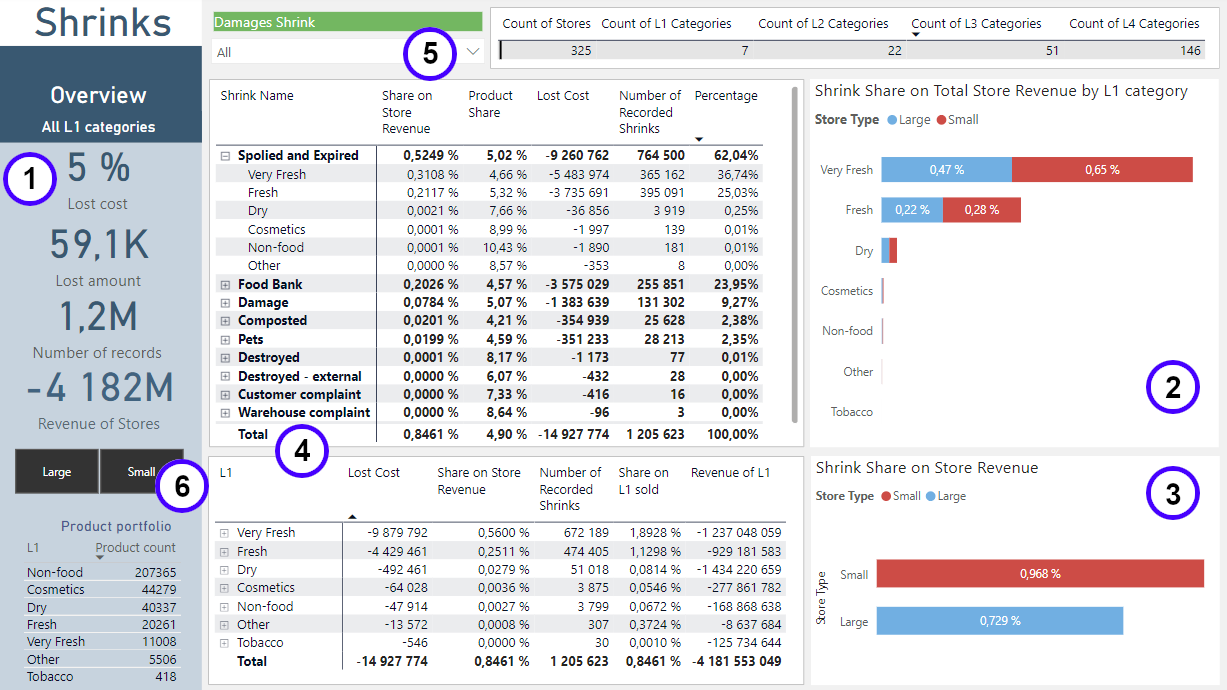
\includegraphics[width=\textwidth]{obrazky/PBI/overview.png}
    \caption{Power BI reporting pro zobrazení údajů o shrincích.}
    \label{obr:PBI:overview}
\end{figure}

Přehledová stránka dále obsahuje dvě tabulky. První tabulka sleduje vybrané ukazatele pro typy shrinků, které lze dále prozkoumat z~pohledu kategorií první úrovně. Druhá tabulka zobrazuje ukazatele z~pohledu kategorií, a to od nejvyšší úrovně po nejnižší, případně až na detail samotných produktů a jejich ID. Vzhledem k~tomu, že tabulka může při detailním procházení zabírat více místa je možné přejít na její detail, který se zobrazí přes celou aktuální stránku. Ukázka této tabulky je na obr.~\ref*{obr:PBI:tab1}.
U čísel 5 a 6 jsou umístěny filtry -- pro typ prodejny a pro typ shrinku. Vyfiltrováním příslušného typu se hodnoty v~reportingu automaticky upraví. Všechny nevybrané kategorie nejsou zahrnuté do vizuálů, ani výpočtů hodnot. Např. pokud uživatel vybere pouze velké prodejny, celkové tržby se týkají již pouze všech velkých prodejen, nejde o celkové tržby všech prodejen z~datasetu.

\begin{figure}[h!]
    \centering
    \captionsetup{justification=centering}
    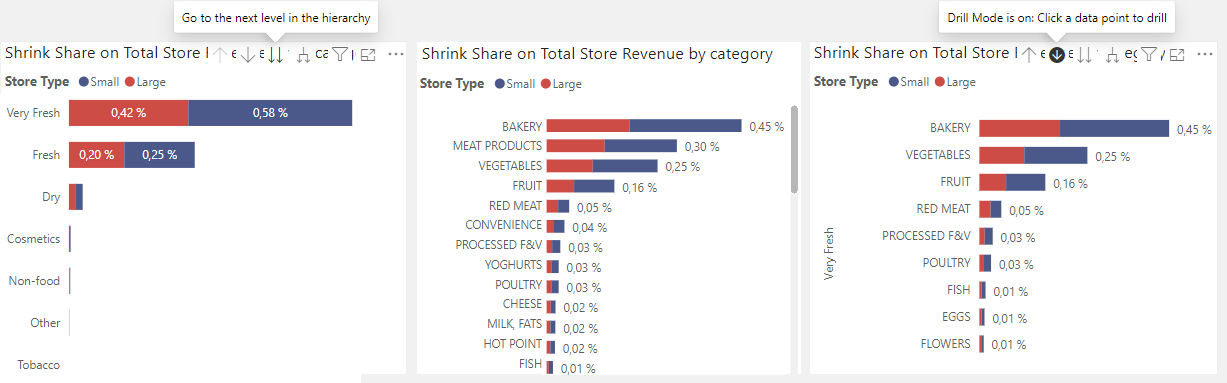
\includegraphics[width=\textwidth]{obrazky/PBI/Catdrilldown.png}
    \caption{Ukázka interakce grafu záznamů shrinku pro přístupy \\ k~různým úrovním produktové hierarchie.}
    \label{obr:PBI:drill}
\end{figure}

\begin{figure}[h!]
    \centering
    \captionsetup{justification=centering}
    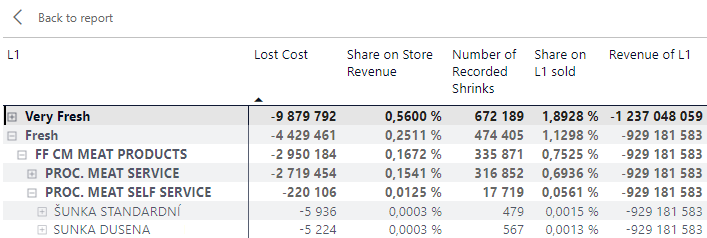
\includegraphics[width=\textwidth]{obrazky/PBI/tabulkaukzka.png}
    \caption{Power BI -- Detail tabulky vybrané ukazatele pro jednotlivé kategorie \\ v~produktové hierarchii.}
    \label{obr:PBI:tab1}
\end{figure}

\subsubsection*{Prodejny}

Další stránka zobrazuje prodejny a k~nim příslušné ukazatele. Uživatel může filtrovat prodejny podle typu, kraje nebo okresu. Dále je možné filtrovat také podle kategorií. V~tabulce lze zobrazit údaje agregovaně podle lokalit nebo přímo pro jednotlivé prodejny. Sloupce tabulky jsou rozdělené na hodnoty týkající se malých nebo velkých prodejen a poté celkové hodnoty pro oba typy. Graf stromová mapa pod číslem 1, obsahuje kraje, resp. vybrané okresy, ve kterých se nachází prodejny. Plocha příslušné lokality zabírá tolik procent obsahu grafu, kolik procent tvoří hodnota shrinků v~této lokalitě. Graf č. 2 porovnává zaznamenaný shrink s~počtem prodejen v~regionu. 
Ukázka této stránky je na obr.~\ref*{obr:PBI:stores}.

\begin{figure}[h!]
    \centering
    \captionsetup{justification=centering}
    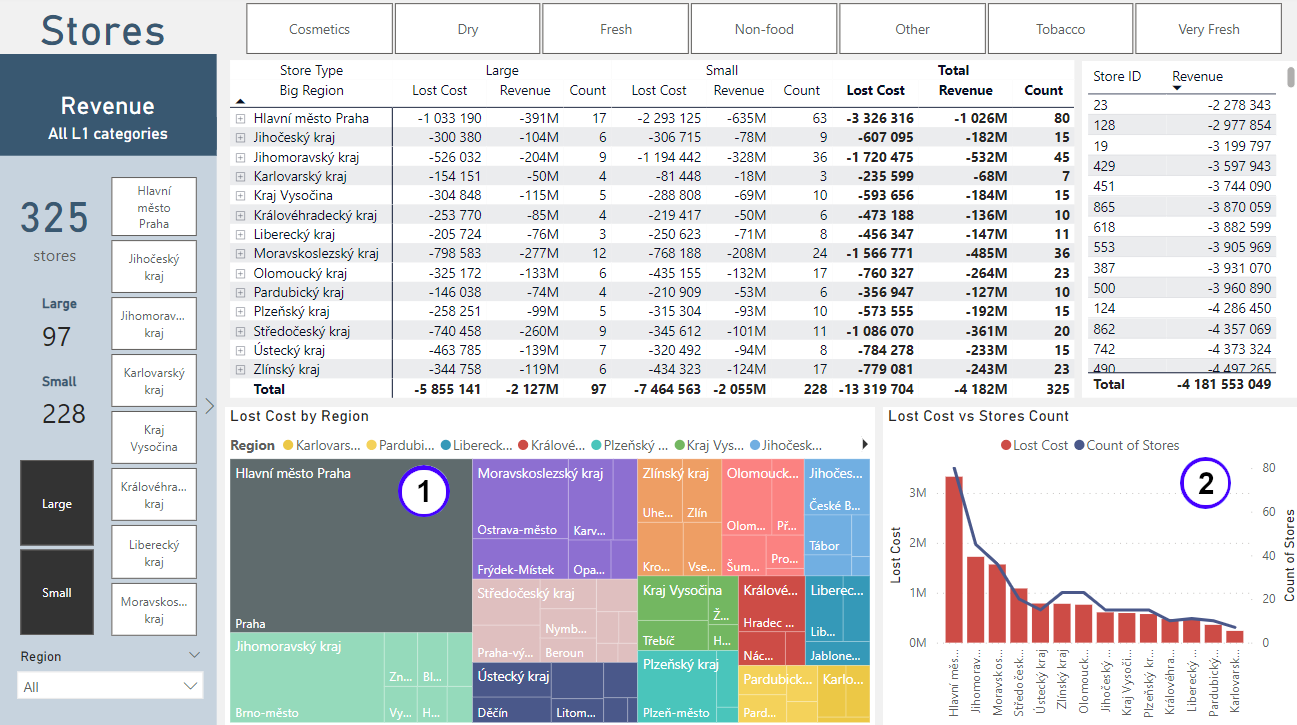
\includegraphics[width=\textwidth]{obrazky/PBI/storesall.png}
    \caption{Power BI reporting pro zobrazení údajů o shrincích z~pohledu prodejen.}
    \label{obr:PBI:stores}
\end{figure}

\subsubsection*{Prodejny -- Velmi čerstvé a Čerstvé}

Na této stránce reportu jsou vizuály pro analýzu chování shrinků z~hlediska prodejen již pouze pro kategorie Čerstvé a Velmi čerstvé viz obr.~\ref*{obr:PBI:storesSFF}. V~nastavení reportu v~sekci filtrů je možné vybrat i další kategorie, nicméně tato práce se věnuje především analýze těchto dvou kategorií, a tak jsou již předfiltrované tyto kategorie. Opět je možné filtrovat prodejny podle jejich atributů. Také je možné v~horní části stránky vybrat sledovaný shrink (č. 1) -- shrinky jsou pro lepší přehlednost barevně odlišené. 
Stránka dále obsahuje graf č. 2, který vizualizuje zastoupení shrinků podle hodnoty shrinku (tj. ztracené náklady). 
 Graf porovnání velkých a malých prodejen podle absolutního zaznamenaného shrinku na všech prodejnách a graf průměrné hodnoty shrinku na prodejně pro oba typy prodejen (č. 3). Pod tímto grafem jsou prodejny porovnané podle jejich ztracených nákladů. Zároveň je datový pruh barevně rozdělený podle typu shrinku (barva je shodná s~barvou shrinku, kterou má přiřazenou nahoře na stránce). 

Graf označený č. 4 zobrazuje ztrátu vlivem shrinku podle velikosti měst, ve kterých se prodejny nachází. Graf umožňuje přejít k~podrobnostem, a to typu prodejny a konkrétním prodejnám. Zbylé grafy na stránce zobrazují konkrétní prodejny podle ukazatelů - hodnota shrinku, podíl shrinku na celkových tržbách prodejny, podíl shrinku na tržbách kategorií Velmi čerstvé a čerstvé na sledované prodejně. Grafy jsou rozdělené podle typu prodejen, datové pruhy jsou opět poměrově rozdělené podle zastoupení typů shrinků.

\begin{figure}[h!]
    \centering
    \captionsetup{justification=centering}
    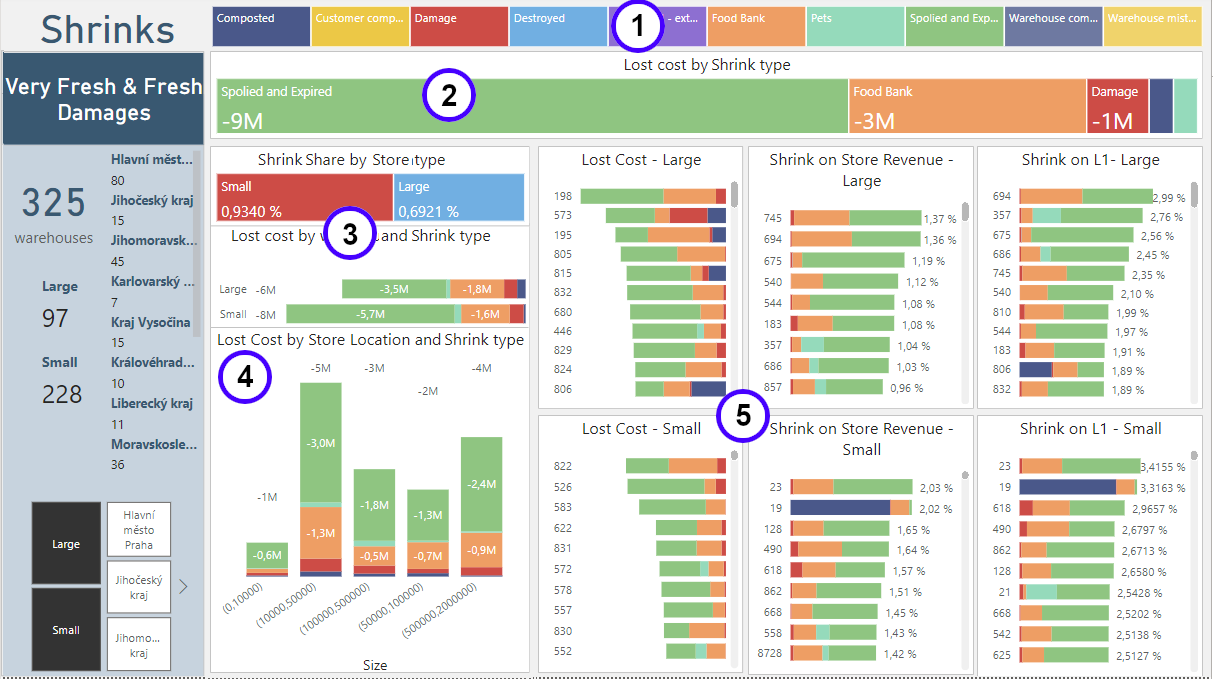
\includegraphics[width=\textwidth]{obrazky/PBI/storesSFF.png}
    \caption{Power BI reporting pro zobrazení údajů o shrincích kategorie \\ Čerstvé a Velmi čerstvé z~pohledu prodejen.}
    \label{obr:PBI:storesSFF}
\end{figure}

\subsubsection*{Kategorie -- Velmi čerstvé a Čerstvé}

Další stránka zobrazuje data kategorií Velmi čerstvé a Čerstvé podle dalších přízna-\\ků. Grafy označené jedničkou zobrazují podíl shrinku na celkových tržbách podle kategorie (z~libovolné úrovně až k~detailu produktu) a také zastoupení typu promoakce produktů v~záznamech, zároveň je datovým pruhům přiřazeno zastoupení typu shrinku. Graf označený dvojkou zobrazuje závislost ztracených nákladů a podílu shrinku na tržbách pouze daného produktu. Zobrazeny jsou pouze ty produkty, kde je ztráta vyšší než daná hodnota a podíl vyšší než 20~\%. Produkty jsou barevně odlišené podle kategorie, do které patří. Tabulka vlevo od grafu 2 říká, kolik unikátních produktů bylo shrinkováno podle typu prodejny, od typu jde dále přejít přes lokaci k~samotným prodejnám. Graf č. 3. ukazuje počet záznamů evidovaných v~daný den v~týdnu, legenda zároveň určuje, v~které části měsíce to bylo. 

\begin{figure}[h!]
    \centering
    \captionsetup{justification=centering}
    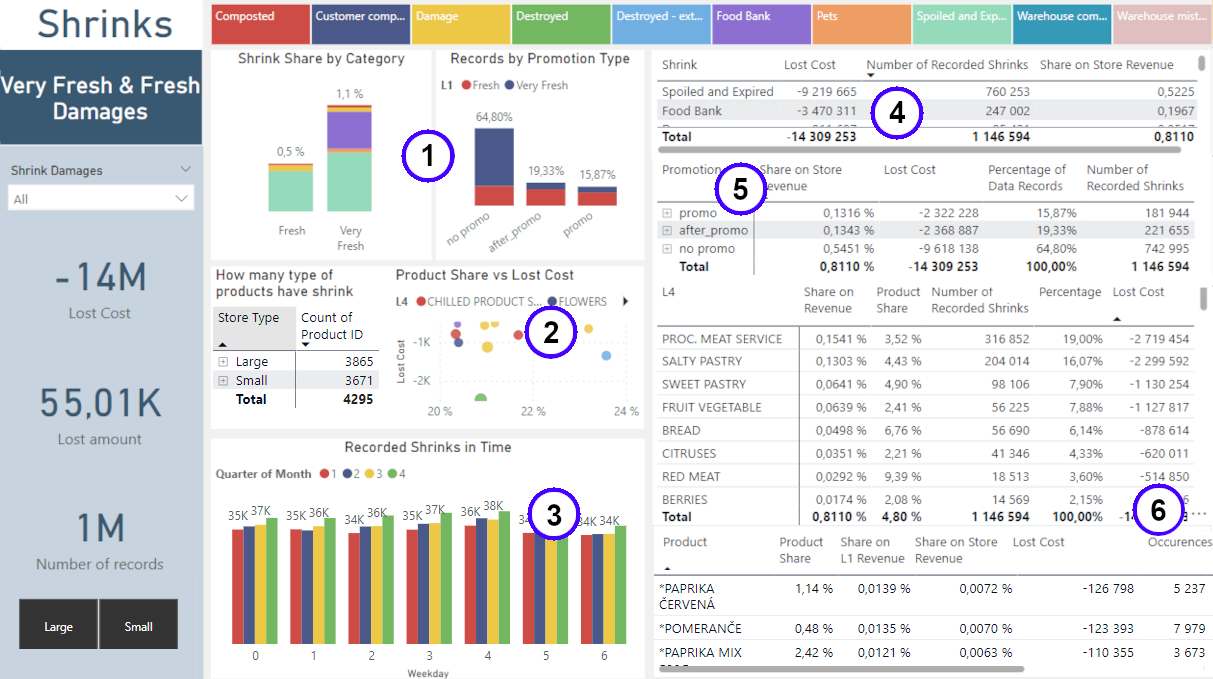
\includegraphics[width=\textwidth]{obrazky/PBI/levelsSFFkopie.png}
    \caption{Power BI -- Zobrazení údajů o shrincích kategorie Čerstvé a Velmi čerstvé \\ se zaměřením na kategorie a produkty.}
    \label{obr:PBI:levelsSFF}
\end{figure}

Tabulka č. 4 přiřazuje vybrané ukazatele k~jednotlivým typům shrinku. Další tabulka obsahuje také tyto údaje ale přiřazené podle typu promoakce produktu, který je evidován v~záznamu shrinku. Následující tabulky se týkají již konkrétních kategorií a produktů, z~produktu se lze přesunout na další stránku věnující se detailu pouze jednoho produktu (viz obr.~\ref*{obr:PBI:drilldetail}). Sledován je podíl shrinku na tržbách prodejny, na tržbách produktu na prodejne, výskyt v~záznamech, ztracená tržba a její procentuální zastoupení. Na stránce jsou i jako v~předešlých případech filtry a souhrnné údaje.

\begin{figure}[h!]
    \centering
    \captionsetup{justification=centering}
    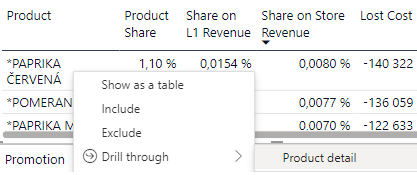
\includegraphics[width=0.45\textwidth]{obrazky/PBI/detaildrill.png}
    \caption{Power BI -- Proklik na stránku s~detailem produktu.}
    \label{obr:PBI:drilldetail}
\end{figure}

\subsubsection*{Čas -- Velmi čerstvé a Čerstvé}

Na další stránce jsou data porovnávána vzhledem k~datu záznamu, tj. ke dni v~týdnu a části měsíce. Na této stránce, kromě filtrování typů jako v~předchozích případech, může uživatel určit pro který ukazatel budou grafy zobrazeny. Vybrat lze ze ztracených nákladů, podílu shrinku na celkových tržbách prodejny a z~podílu shrinku na tržbách v~dané kategorii a případně v~části měsíce, viz č. 1 na obr.~\ref*{obr:PBI:timeSFF}. Zbylé grafy jsou rozděleny na tři části -- podle typu shrinku, podle umístění prodejen a podle typu prodejny. V~každé části je přehled, který říká v~jakém poměru tyto příznaky jsou (v~závislosti na zvoleném ukazateli). Každá část zobrazuje poměry v~porovnání s~dny v~ týdnu, resp. s~částmi měsíce.

\begin{figure}[h!]
    \centering
    \captionsetup{justification=centering}
    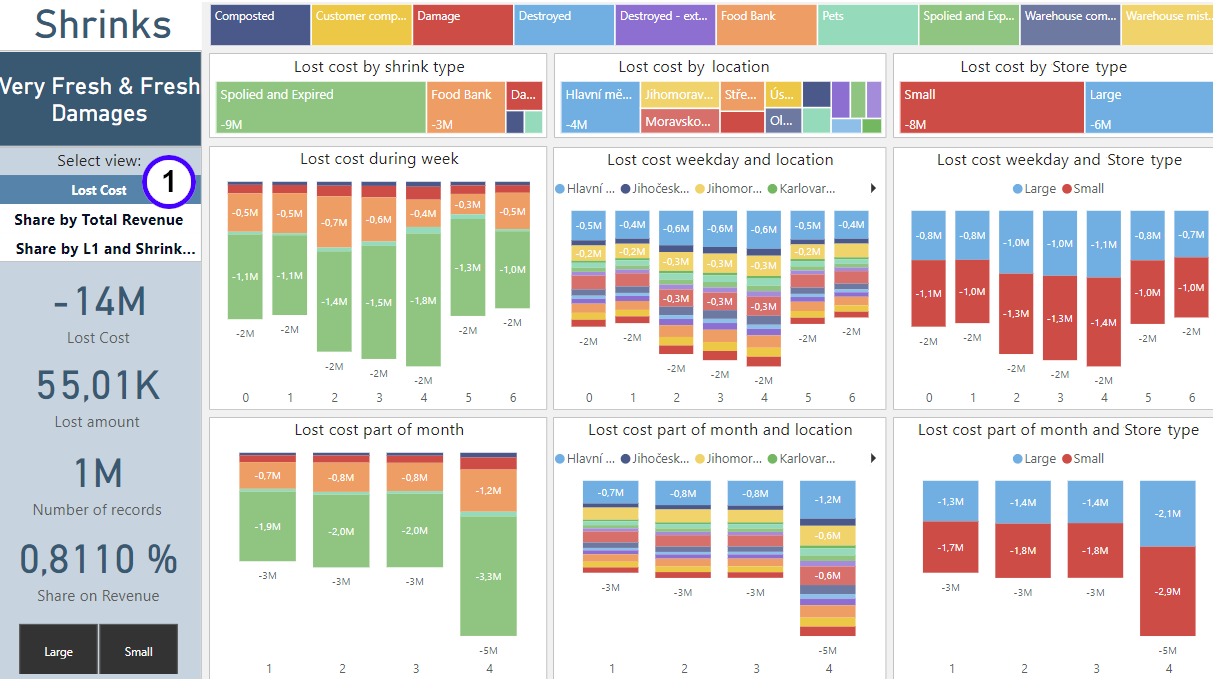
\includegraphics[width=\textwidth]{obrazky/PBI/timeSFF.png}
    \caption{Power BI -- Zobrazení údajů o shrincích kategorie Čerstvé a Velmi čerstvé \\ se zaměřením na časové údaje.}
    \label{obr:PBI:timeSFF}
\end{figure}

\subsubsection*{Detail produktu}

Poslední stránka je věnovaná analýze konkrétního produktu, snímek je na obr. \ref*{obr:PBI:detail}. Je zobrazené zastoupení produktu podle typu prodejny a podle kraje z~pohledu ztracených nákladů (č. 1). Dále je na této stránce tabulka (č. 2) se záznamy agregovaná podle data záznamu. Každý řádek s~datem lze dále rozbalit pro detail o jaký typ shrinku se jednalo, k~jednotlivým řádkům jsou napočítané vybrané ukazatele. Další tabulka (č. 3) ukazuje, jaký podíl na tržbách produktu a celkových tržbách má který typ shrinku. 

Zbylé grafy ukazují konkrétní prodejny, které měly největší podíl shrinku tohoto produktu na svých tržbách, opět celkových i produktových. Dále jak je shrink tohoto produktu rozložený do dní v~týdnu, resp. do částí v~měsíci (č. 4).

\begin{figure}[h!]
    \centering
    \captionsetup{justification=centering}
    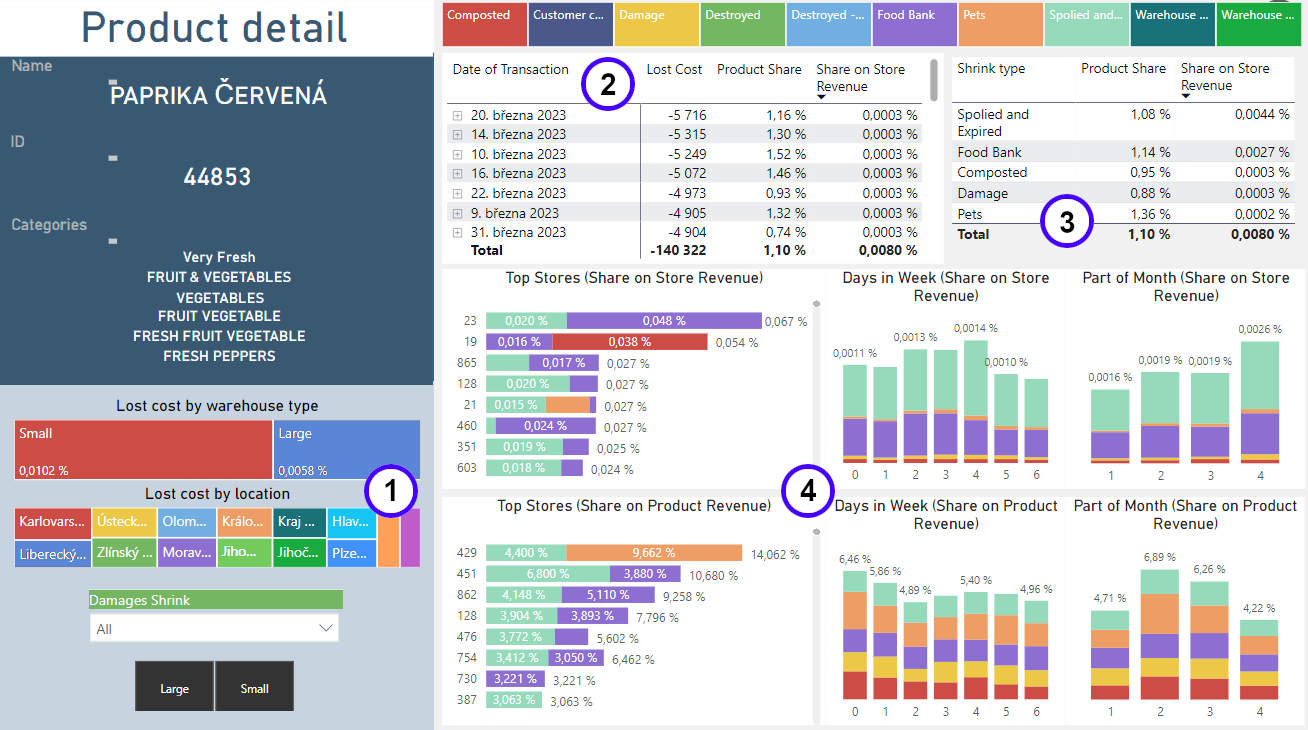
\includegraphics[width=\textwidth]{obrazky/PBI/productdetail.png}
    \caption{Power BI report -- Detail produktu.}
    \label{obr:PBI:detail}
\end{figure}

\section{Výsledky}
\label{sec:vizualizace:vysl}

Díky Power BI reportu je možné snadno zjistit, které kategorie či produkty jsou zastoupené více než jiné, nebo které prodejny mají vysoký podíl shrinku na svých tržbách a v~jakém okrese ke shrinkům dochází nejčastěji. Tato sekce obsahuje popis zjištěných informací z~dat, a to včetně ukázek konkrétních vizualizací, ze kterých pozorování vychází.
První část se věnuje pozorování na celých datech. tj. pozorovaná data za měsíc březen roku 2023, všech evidovaných shrinků způsobených škodami. Druhá část popisuje chování produktů v~kategorii Čerstvé a Velmi čerstvé a typu shrinku prošlé a zkažené zboží.

\subsection*{Pozorování na celých datech}

Pořadí zastoupení shrinků jednotlivých kategorií první úrovně hierarchie na celkových tržbách v~datech lze vidět na obrázku \ref*{obr:PBI:vysL1}. Je vidět, že kategorie Velmi čerstvé a Čerstvé jsou výrazně více zastoupeny než zbylé kategorie. Na témže obrázku se nachází i porovnání hodnot vzhledem k~velikosti prodejen. 
Malé prodejny mají v~kategoriích s~nejvyšším podílem shrinků na tržbách větší podíl než velké prodejny.
Na následujícím obrázku \ref*{obr:PBI:vysL34} je zobrazeno zastoupení kategorií třetí a čtvrté úrovně opět s~porovnáním pro oba typy prodejen. Všechny zobrazené kategorie jsou podkategoriemi skupin Velmi čerstvé nebo Čerstvé.

\begin{figure}[h!]
    \centering
    \captionsetup{justification=centering}
    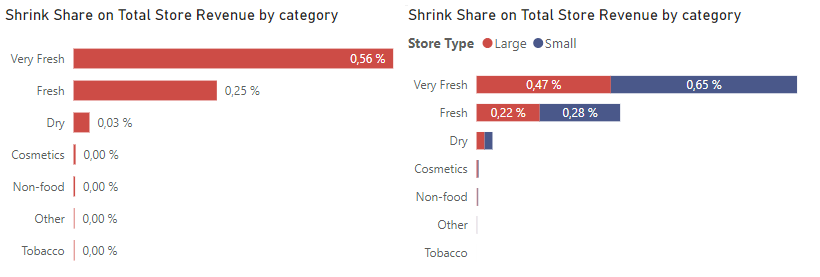
\includegraphics[width=\textwidth]{obrazky/PBI/vys_L1.png}
    \caption{Power BI report -- Zastoupení kategorií na celkových tržbách  \\ ve sledovaném období (vlevo) a porovnání vzhledem k~velikosti prodejen (vpravo).}
    \label{obr:PBI:vysL1}
\end{figure}

\begin{figure}[h!]
    \centering
    \captionsetup{justification=centering}
    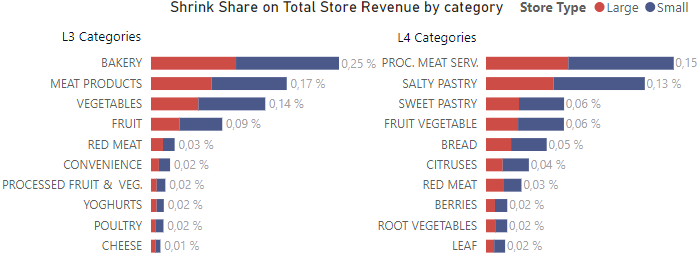
\includegraphics[width=\textwidth]{obrazky/PBI/l3l4.png}
    \caption{Power BI report -- Zastoupení kategorií 3. a 4. úrovně \\na celkových tržbách ve sledovaném období.}
    \label{obr:PBI:vysL34}
\end{figure}


Tabulka \ref*{tab:PBI:vysL1} obsahuje agregované důležité metriky podle sedmi hlavních kategorií. Kategorie Velmi čerstvé má nejvíce evidovaných záznamů, rovněž nejvyšší oba podíly na tržbách i největší celkovou ztrátu způsobenou shrinkem. Hodnota shrinku činí téměř dvě procenta tržeb kategorie. Co se týče tržeb za tuto kategorii, jedná se o druhou kategorii s~nejvyššími tržbami ve sledovaném období. Vyšší tržby má pouze kategorie Suché, kde ale relativní ztráta u tohoto typu zboží je více než dvacetkrát menší. Kategorie Čerstvé se vyskytuje téměř v~půl milionu záznamů. Hodnota shrinků produktů je více než jedno procento tržeb této kategorie. Zbylé kategorie mají velmi malé zastoupení v~datech a význam vzhledem ke svým tržbám.

\begin{table}[!h]
    \centering
    \caption{Tabulka základních metrik pro kategorie první úrovně produktové hierarchie.}
    \begin{tabular}{l rrrrr}
        Kategorie & \vtop{\hbox{\strut Hodnota}\hbox{\strut shrinku}}  & \vtop{\hbox{\strut Počet}\hbox{\strut záznamů}}  &  \vtop{\hbox{\strut Podíl na }\hbox{\strut tržbách}\hbox{\strut  kategorie [\%]}} & \vtop{\hbox{\strut Podíl na }\hbox{\strut celkových}\hbox{\strut  tržbách [\%]}}& \vtop{\hbox{\strut Tržby}\hbox{\strut kategorie}}  \\ 
        \midrule
        Velmi čerstvé & $9\,879\,792$ & $672\,189$ & $1{,}8928$ & $0{,}5600$ & $1\,23 7\, $mil. \\ %048\,059$ \\ 
        Čerstvé & $4\,429\,461$ & $474\,405$ & $1{,}1298$ & $0{,}2511$ & $929\, $mil. \\ %181\,583$ \\ 
        Suché & $492\,461$ & $51\,018$ & $0{,}0814$ & $0{,}0279$ & $1\,434\, $mil. \\ %220\,659$ \\ 
        % \vtop{\hbox{\strut Kosmetika}\hbox{\strut  a drogerie}} & $64\,028$ & $3\,875$ & $0{,}0546$ & $0{,}0036$  & $277\, $mil. \\ %861\,782 $\\ 
        Kosmetika a drogerie & $64\,028$ & $3\,875$ & $0{,}0546$ & $0{,}0036$  & $277\, $mil. \\ %861\,782 $\\ 
        Nepotravinářské & $47\,914$ & $3\,799$ &$ 0{,}0672$ & $0{,}0027$  & $168\, $mil. \\ %868\,638$ \\ 
        Ostatní & $13\,572$ & $307$ & $0{,}3724$ & $0{,}0008$ & $8\, $mil. \\ %637\,684$ \\ 
        Tabák & $546$ & $30$ &$ 0{,}0010$ & $0{,}0000$  & $125\, $mil. \\ %734\,644$ \\ 
    \end{tabular}
    \label{tab:PBI:vysL1}
\end{table}

Další tabulka \ref*{tab:PBI:vysSh} obsahuje hodnoty ukazatelů k~jednotlivým typům shrinků. Lze vidět, že Prošlé a zkažené zboží tvoří 62~\% všech shrinků z~pohledu ztracených nákladů. Necelými 24~\% jsou zastoupené produkty, které byly věnovány potravinovým bankám. Jedná se sice o druhý nejčastější shrink v~záznamech, nicméně toto zboží není vyhozeno zcela, ale je předáno dále. Pro společnost se jedná stále ztracený zisk, ale zboží je dál efektivně využito a nedochází tak k~plýtvání jako takovému. Další typy shrinků dohromady netvoří ani 15~\% všech ztracených nákladů. Potravinová banka je evidována z~96~\% u produktů z~kategorie Velmi čerstvé a jedná se především o podkategorie Pečivo (62~\%), Zelenina (19~\%) a Ovoce ($12{,}5$~\%).

\begin{table}[h!]
    \centering
    \caption{Tabulka základních metrik pro jednotlivé typy shrinků.}
\begin{tabular}{lrrrrr}
Typ shrinku          & \vtop{\hbox{\strut Hodnota}\hbox{\strut shrinku}}  & \vtop{\hbox{\strut Počet}\hbox{\strut záznamů}}  &  \vtop{\hbox{\strut Průměr. podíl}\hbox{\strut na  tržbách}\hbox{\strut  produktů [\%]}} & \vtop{\hbox{\strut Podíl na }\hbox{\strut celkových}\hbox{\strut tržbách [\%]}}& \vtop{\hbox{\strut Hodnota}\hbox{\strut shrinku}\hbox{\strut [\%]}}  \\ 
\midrule
\vtop{\hbox{\strut Prošlé}\hbox{\strut a zkažené zboží}}        & $9\,260\,762$  & $764\,500$ & 5{,}02    & 0{,}5249    & 62{,}04\\
\vtop{\hbox{\strut Potravinová}\hbox{\strut banka}}             & $3\,575\,029$  & $255\,851$ & 4{,}57    & 0{,}2026    & 23{,}95\\
   \vtop{\hbox{\strut Poškození}\hbox{\strut  }}                & $1\,383\,639$  & $131\,302$ & 5{,}07    & 0{,}0784    & 9{,}27 \\
   \vtop{\hbox{\strut Kompostéry}\hbox{\strut  }}               & $354\,939$   & $25\,628$  & 4{,}21    & 0{,}0201    & 2{,}38 \\
\vtop{\hbox{\strut Zvířecí}\hbox{\strut útulky}}                & $351\,233$   & $28\,213$  & 4{,}59    & 0{,}0199    & 2{,}35 \\
    \vtop{\hbox{\strut Zničení}\hbox{\strut  }}                 & $1\,173$     & $77 $    & 8{,}17    & 0{,}0001    & 0{,}01 \\
\vtop{\hbox{\strut Poškození}\hbox{\strut vnějšími  vlivy}}     & $432$      & $28$     & 6{,}07    & 0{,}0000    & 0{,}00 \\
\vtop{\hbox{\strut Zákaznické}\hbox{\strut reklamace}}          & $416$      & $16$     & 7{,}33    & 0{,}0000    & 0{,}00 \\
\vtop{\hbox{\strut Reklamace}\hbox{\strut centrálního skladu}}  & $96$       & $3$      & 8{,}64    & 0{,}0000    & 0{,}00 \\
% Warehouse mistake    & $56$       & $5$      & 1{,}86    & 0{,}0000   & 0{,}00
\end{tabular}
\label{tab:PBI:vysSh}
\end{table}

Obrázek \ref*{obr:PBI:loc} obsahuje graf typu stromová mapa. Na grafu jsou zobrazeny kraje České republiky, případně okresy s~nejvyššími hodnotami shrinku. Pole příslušného kraje zabírá tolik procent grafu, kolik zaujímá evidovaný shrink. Necelých 25~\% z~celkového hodnoty všech zaznamenaných shrinků patří do kraje Hlavní město Praha. Dalších téměř 25~\% tvoří kraje Jihomoravský a Moravskoslezský v~podobném poměru. Největší zastoupení v~těchto krajích mají okresy příslušející jejich krajským městům. Záznamy ze Středočeského kraje tvoří $8{,}2$~\% ztracených nákladů. Každý z~krajů Zlínský, Ústecký, Olomoucký tvoří necelých $6$~\%. Zbylé kraje jednotlivě zaujímají méně jak $5$~\% na celkovém shrinku. Na grafu \ref*{obr:PBI:locvs} je porovnání hodnoty shrinku a počtu prodejen pro kraje, je vidět, že tyto dva ukazatele spolu souvisí.

\begin{figure}[h!]
    \centering
    \captionsetup{justification=centering}
    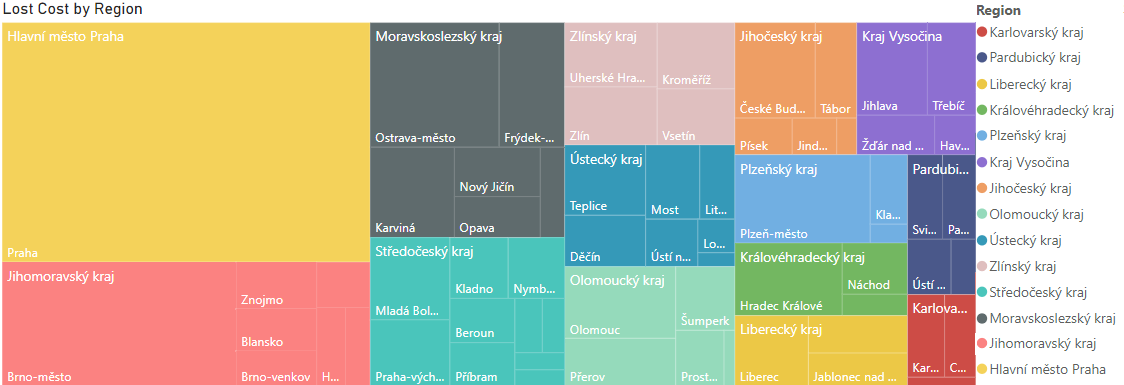
\includegraphics[width=\textwidth]{obrazky/PBI/location.png}
    \caption{Power BI report -- Zobrazení krajů podle velikosti hodnoty shrinku (vlevo) a počet prodejen v~regionu (vpravo).}
    \label{obr:PBI:loc}
\end{figure}

Na dalším obrázku \ref*{obr:PBI:norm} jsou zobrazeny průměrné údaje na jednu prodejnu v~daném kraji. Porovnána je průměrná velikost shrinku na prodejně a podíl tohoto shrinku na průměrných tržbách v~kraji. Z~grafu lze vidět, že podle průměrných hodnot v~krajích: Olomoucký, Pardubický a Plzeňský. V~těchto oblastech je podíl shrinku na tržbách výrazně nižší než v~jiných krajích. V~těchto třech krajích a ještě v~ Karlovarském a Zlínském kraji je průměrná hodnota shrinku nižší u ostatních krajů. Nejvyšší hodnoty podílů jsou pro kraje Karlovarské, Královehradecký, Ústecký. Průměrná hodnota shrinku je nejvyšší u krajů Středočeský a Ústecký. 
Data se týkají všech shrinků způsobených škodami a celého produktového portfolia.

Na základě dvou předešlých pozorování by bylo vhodné se zaměřit na prodejny v~Karlovarském a Královehradeckém kraji.

\begin{figure}[h!]
    \centering
    \captionsetup{justification=centering}
    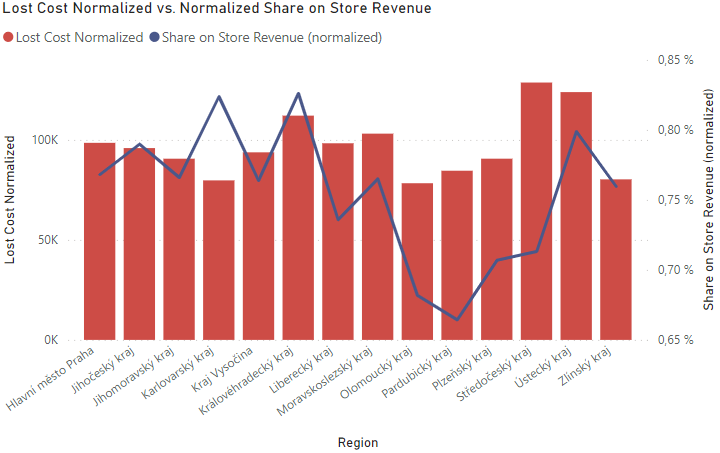
\includegraphics[width=\textwidth]{obrazky/PBI/normalized.png}
    \caption{Power BI report -- Zobrazení krajů podle průměrné hodnoty shrinku na jednu prodejnu v porovnání s podílem shrinku na průměrných tržbách kraje.}
    \label{obr:PBI:norm}
\end{figure}


Na obrázku \ref*{obr:PBI:types} nahoře je zobrazen jaký je podíl celkového shrinku na tržbách všech prodejen daného typu. V~dolní části je poměr normalizované hodnoty shrinku na prodejnách obou typů -- tj. průměrně jedna velká prodejna  tvoří 65~\% evidovaných shrinků, zatímco malé prodejny zbylých 35~\%.

\begin{figure}[hbtp!]
    \centering
    \begin{minipage}{.5\textwidth}
        \centering
        \captionsetup{justification=centering}
        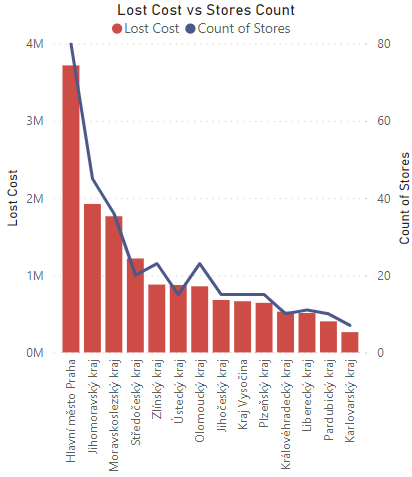
\includegraphics[width=\textwidth]{obrazky/PBI/vsLoc.png}
        \caption{Power BI report -- Porovnání hodnoty shrinku a počtu prodejen \\pro jednotlivé kraje.}
        \label{obr:PBI:locvs}
    \end{minipage}%
    \begin{minipage}{.5\textwidth}
        \centering
        \captionsetup{justification=centering}
        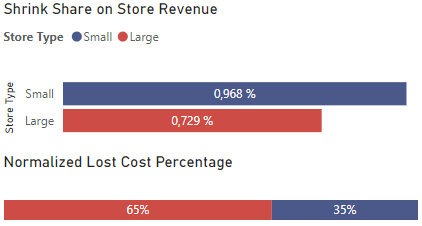
\includegraphics[width=\textwidth]{obrazky/PBI/normTypes.png}
        \caption{Power BI report -- Porovnání typů prodejen z~hlediska podílu shrinku na tržbách (nahoře) a průměrné velikosti shrinku jedné prodejny v~kategorii.}
        \label{obr:PBI:types}
    \end{minipage}
\end{figure}

Pro většinu prodejen platí, že největší část hodnoty zaznamenaných shrinků tvoří prošlé a zkažené zboží, případně zboží darované potravinové bance. Neobvyklé zastoupení shrinků ale vykazují malé prodejny s~ID 19 (Brno) a 126 (okres Třebíč), kdy největší část zboží je kompostována a téměř žádné není vyhozeno jako shrink prošlého zboží. Ukázka grafů je na obrázku \ref*{obr:PBI:topwhs}. V~levé části obrázku jsou dva grafy. Jeden zobrazuje průměrnou hodnotu shrinku pro jednu prodejnu, a tedy i průměrné zastoupení typů shrinku. Druhý obsahuje součet hodnot shrinků přes všechny prodejny.

\begin{figure}[h!]
    \centering
    \captionsetup{justification=centering}
    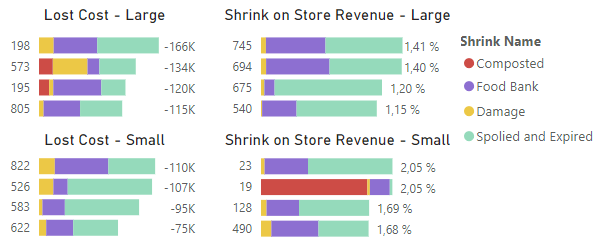
\includegraphics[width=\textwidth]{obrazky/PBI/topwhs.png}
    \caption{Power BI report -- Hodnota shrinku pro typ prodejny). Prodejny s~nejvyšší hodnotou ukazatelů (vpravo) -- ztracené náklady a podíl shrinku na tržbách.}
    \label{obr:PBI:topwhs}
\end{figure}

\subsection*{Pozorování pro vybraná data}

Tato část se věnuje pouze datům, která se týkají kategorií Velmi čerstvé a Čerstvé a shrinku prošlé a zkažené zboží. Evidovaný shrink má pouze na těchto kategoriích hodnotu $9{,}2$ mil. peněžních jednotek. 
Na grafu \ref*{obr:PBI:porovnani} je vidět, že malé prodejny mají ve většině nižší hodnotu shrinku, ale podíl na shrinku na tržbách mají vyšší než velké prodejny. Prodejny s~velmi nízkými shrinky mají i nízký podíl shrinku na tržbách. 
Největší ztracené náklady byly evidovány u velké prodejny s~ID 198 v~Praze, nicméně podíl tohoto shrinku na celkových tržbách je pouhých $0{,}23$~\%, což je jeden z~nejnižších. Zároveň se jedná o prodejnu s~nejvyššími tržbami. Zatímco velká prodejna 675 v~okresu Uherské Hradiště má třetí nejvyšší hodnotu shrinku a zároveň i nejvyšší podíl shrinku na tržbách $1{,}68$~\% mezi velkými prodejnami. 
Nejvyšší podíl shrinku na svých tržbách byl evidován u malé prodejny 23, které se nachází v~Brně, nicméně hodnota shrinku je nízká. Druhý nejvyšší podíl má malá pražská prodejna.
Z~grafu je patrné, že čtyři malé prodejny mají podobné tržby jako velké prodejny. Jedná se o dvě prodejny v~Praze a prodejny v~okresu Litoměřice a Jablonec nad Nisou, tyto pražské prodejny mají vyšší podíl shrinku než zbylé dvě prodejny.
Z~hlediska umístění prodejen do krajů a okresů nebyl v~datech na této úrovni detailu objeven žádný vzor.

\begin{figure}[h!]
    \centering
    \captionsetup{justification=centering}
    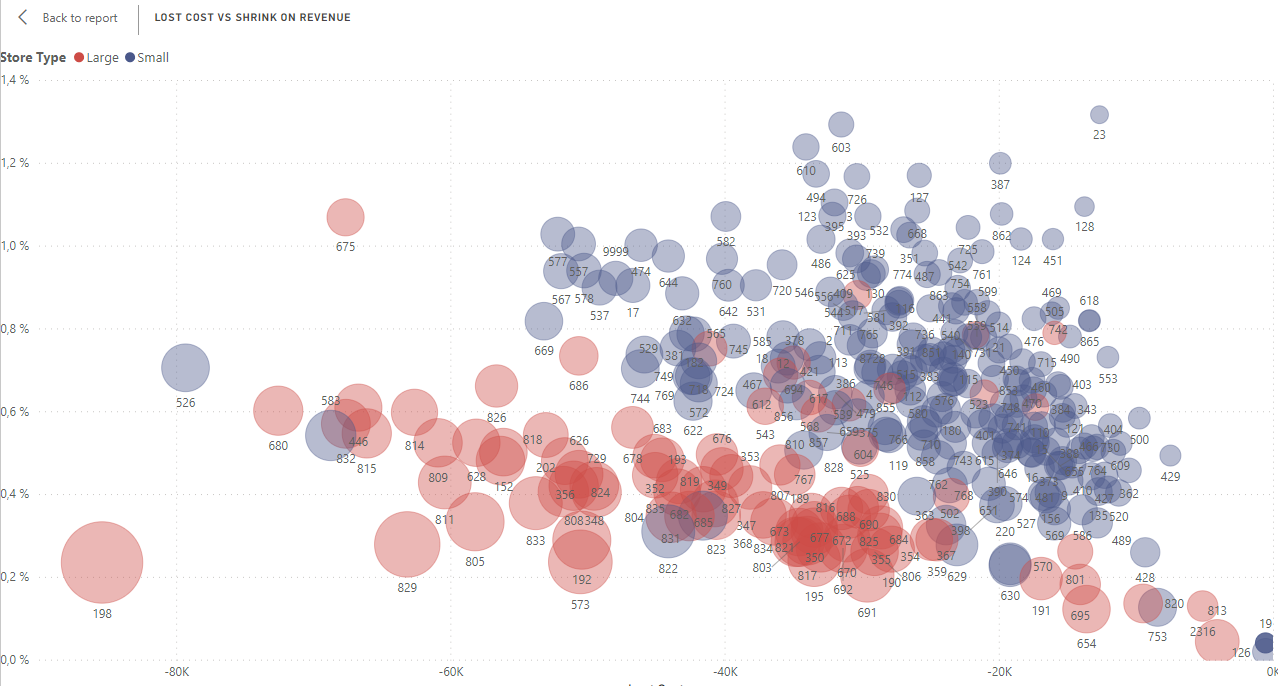
\includegraphics[width=\textwidth]{obrazky/PBI/porovnaniprodejen.png}
    \caption{Power BI report -- Velikost shrinku na prodejně versus podíl shrinku\\ na tržbách. Velikost zobrazeného bodu ukazuje výši tržeb na prodejně}
    \label{obr:PBI:porovnani}
\end{figure}

Graf \ref*{obr:PBI:velikost} zobrazuje průměrnou hodnotu shrinků na prodejně podle obydlenosti města, kde se nachází. Pro malé prodejny velikosti shrinku nejsou příliš rozdílné vzhledem k~počtu obyvatel, kde se prodejna nachází. Pro velké prodejny platí, že ve městech do deseti tisíc obyvatel bývá hodnota shrinku vyšší než ve  městech s~více obyvateli.

\begin{figure}[h!]
    \centering
    \captionsetup{justification=centering}
    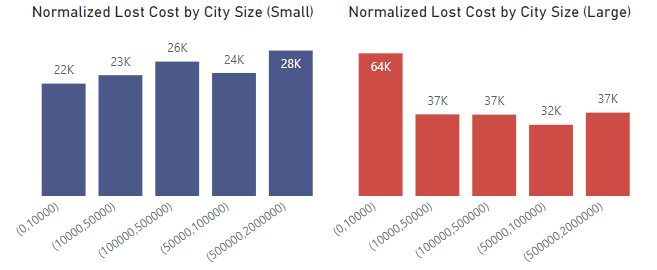
\includegraphics[width=.8\textwidth]{obrazky/PBI/citysize.png}
    \caption{Power BI report -- Průměrná hodnota shrinku prodejen \\ podle velikosti měst, ve které se nachází prodejna.}
    \label{obr:PBI:velikost}
\end{figure}

Z~pohledu času záznamu, tj. dne v~týdnu a čtvrtiny měsíce platí, že nejvyšší shrinky jsou evidovány poslední čtvrtinu měsíce. Důvodem může být to, že část výrobků má datum expirace uvedené ve formátu měsíc-rok, což znamená, že zboží prochází posledním dnem v~měsíci. Dalším důvodem může být, že před začátkem nového měsíce zaměstnanci  evidují více záznamů. Například se může jednat i o shrinky, které se uskutečnili dříve, ale až s~koncem měsíce byly nahrány do systému. Nejvyšší hodnota shrinků je evidována v~pátek, zatímco nejnižší v~neděli, pondělí a úterý. Viz graf \ref*{obr:PBI:time}.

\begin{figure}[h!]
    \centering
    \captionsetup{justification=centering}
    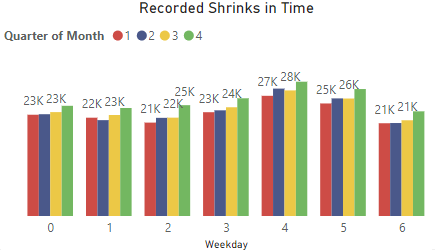
\includegraphics[width=.6\textwidth]{obrazky/PBI/time.png}
    \caption{Power BI report -- Počet záznamů vzhledem ke dni v~týdnu a čtvrtině měsíce.}
    \label{obr:PBI:time}
\end{figure}

Na grafu \ref*{obr:PBI:promo} je procentuální zastoupení evidovaných shrinků vzhledem k~typu promoakce. Nejvíce záznamů se týká produktů bez promoakce, zároveň lze vidět, že Velmi čerstvé  produkty byly ve sledovaném období v~promoakci méně než Čerstvé produkty.

\begin{figure}[h!]
    \centering
    \captionsetup{justification=centering}
    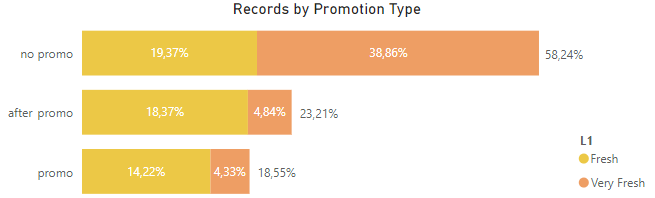
\includegraphics[width=.8\textwidth]{obrazky/PBI/promotype.png}
    \caption{Power BI report -- Počet záznamů podle typu promoakce \\ shrinkovaného produktu.}
    \label{obr:PBI:promo}
\end{figure}

Nejvíce záznamů mají kategorie (úroveň 3) -- Masné výrobky -- pultový prodej (250 tis. záznamů s~hodnotou shrinku 2 mil. peněžních jednotek), Slané a sladké pečivo (127 tis. záznamů s~hodnotou shrinku $1{,}5$ mil. peněžních jednotek), Plodová zelenina (29 tis. záznamů), Chléb (24 tis. záznamů) a Citrusy (22 tis. záznamů). 

\begin{figure}[h!]
    \centering
    \captionsetup{justification=centering}
    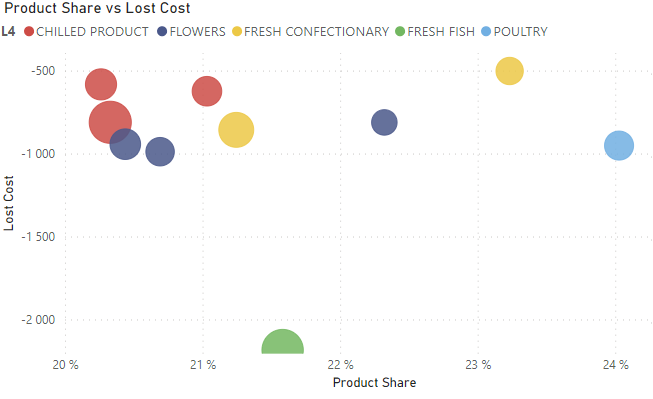
\includegraphics[width=.8\textwidth]{obrazky/PBI/l3pprductshare.png}
    \caption{Power BI report -- Ztracené náklady (hodnota shrinku) vs Podíl shrinku produktu na tržbách produktu. Velikost bodů odpovídá počtu záznamů.}
    \label{obr:PBI:l3prod}
\end{figure}

Produktem, který má nejvyšší zaznamenanou celkovou hodnotu shrinku je balená šunka Nejvyšší jakosti z~kategorie Masných produktů, většina záznamů pochází z~období během promoakce. Druhý nejvyšší shrink měla Dušená šunka nejvyšší jakosti také s~nejvíce záznamy v~promoakci. Oba produkty měly podíl shrinku na svých tržbách téměř 3~\%.  
Nejvyšší podíl na svých tržbách se týká části výrobků z~kategorie sýrů (třetí úroveň hierarchie), podíl se pohybuje okolo 27~\%. Nicméně ztracené náklady nedosahují ani 50 peněžních jednotek a mají jen velmi málo záznamů, podíl na celkových tržbách je tedy zanedbatelný.
Na obr. \ref*{obr:PBI:l3prod} jsou vyfiltrované produkty, které mají hodnotu shrinku větší než 500 peněžních jednotek a zároveň podíl shrinku na svých tržbách více jak 20~\%. Jedná se o tři chlazené produkty, dva produkty z~kategorie cukrovinek, tři druhy řezaných květin, jeden prémiový drůbeží steak a čerstvá treska. 
Nejvyšší podíl na celkových tržbách měly opět tyto dva produkty, dále pak pomeranče, které byly během záznamů shrinků v~promoakci nebo těsně po promoakci.